\documentclass[tikz,border=8pt]{standalone}\usepackage{helvet}\renewcommand{\familydefault}{\sfdefault}\usetikzlibrary{arrows.meta,positioning}\begin{document}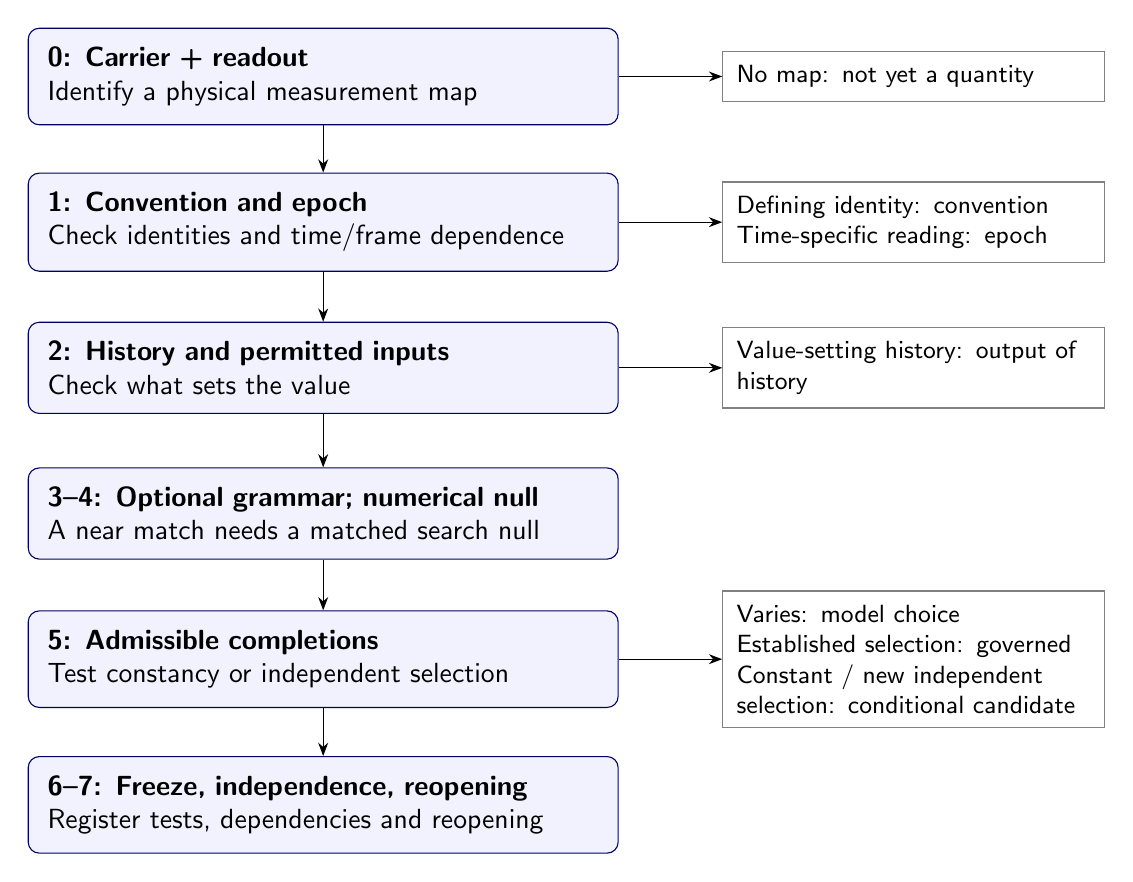
\begin{tikzpicture}
\tikzset{box/.style={draw=blue!40!black,fill=blue!5,rounded corners,text width=7cm,align=left,inner sep=7pt},exit/.style={draw=gray,text width=4.5cm,align=left,inner sep=5pt,font=\small}}
\node[box] (s0) at (0,-0.0) {\textbf{0: Carrier + readout}\\Identify a physical measurement map};
\node[exit] (e0) at (7.5,-0.0) {No map: not yet a quantity};
\draw[-{Stealth}] (s0.east)--(e0.west);
\node[box] (s1) at (0,-1.85) {\textbf{1: Convention and epoch}\\Check identities and time/frame dependence};
\draw[-{Stealth}] (s0.south)--(s1.north);
\node[exit] (e1) at (7.5,-1.85) {Defining identity: convention\\Time-specific reading: epoch};
\draw[-{Stealth}] (s1.east)--(e1.west);
\node[box] (s2) at (0,-3.7) {\textbf{2: History and permitted inputs}\\Check what sets the value};
\draw[-{Stealth}] (s1.south)--(s2.north);
\node[exit] (e2) at (7.5,-3.7) {Value-setting history: output of history};
\draw[-{Stealth}] (s2.east)--(e2.west);
\node[box] (s3) at (0,-5.550000000000001) {\textbf{3--4: Optional grammar; numerical null}\\A near match needs a matched search null};
\draw[-{Stealth}] (s2.south)--(s3.north);
\node[box] (s4) at (0,-7.4) {\textbf{5: Admissible completions}\\Test constancy or independent selection};
\draw[-{Stealth}] (s3.south)--(s4.north);
\node[exit] (e4) at (7.5,-7.4) {Varies: model choice\\Established selection: governed\\Constant / new independent selection: conditional candidate};
\draw[-{Stealth}] (s4.east)--(e4.west);
\node[box] (s5) at (0,-9.25) {\textbf{6--7: Freeze, independence, reopening}\\Register tests, dependencies and reopening};
\draw[-{Stealth}] (s4.south)--(s5.north);
\end{tikzpicture}\end{document}
